%!TEX root = Progetto.tex
\section{Progettazione Concettuale}
	
	\subsection{Strategia di Progetto}
		
		Svilupperemo lo schema concettuale utilizzando in modo intensivo la tecnica di progettazione nota come \emph{Inside-Out}, mischiandola con la strategia \emph{Top-Down}. Partiremo da un'iniziale individuazione di uno scheletro del modello concettuale, quindi procederemo a successive raffinazioni delle componenti che condurranno alla definizione completa del diagramma ER.
		
	\subsection{Individuazione dello Scheletro dello Schema ER}
		
		Dalle specifiche che abbiamo formulato risulta che uno dei punti fondamentali da affrontare è quello della memorizzazione dei preventivi emessi dall'attività.
		Ad ogni \emph{Prestazione} effettuata, corrisponde un \emph{Preventivo} precedentemente emesso.
		
		\begin{figure}[H]
			\centering
			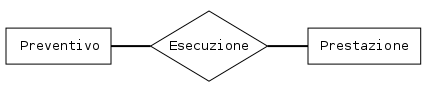
\includegraphics[width=9cm]{images/diagrams/preventivo_prestazione.png}
		\end{figure}
		
		Alla formulazione di ogni preventivo, si fa una stima dei componenti che si reputa saranno necessari per eseguire la prestazione preventivata. Non sempre tale previsione è completamente esatta, generalmente i componenti effettivamente utilizzati in una prestazione sono diversi da quelli previsti in un preventivo.
		L'associazione tra i \emph{Componenti} e il \emph{Preventivo} risulta immediata.
		
		\begin{figure}[H]
			\centering
			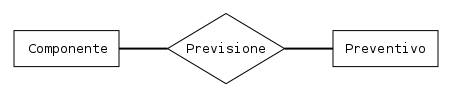
\includegraphics[width=9cm]{images/diagrams/preventivo_componente.png}
		\end{figure}
		
		Prima di esplicitare l'associazione tra le prestazioni eseguite ed i componenti effettivamente utilizzati, affrontiamo la questione degli ordini e del magazzino.
		
		L'acquisto di articoli presso un fornitore è formalizzato in un ordine, il quale, come da specifiche, è organizzato in più forniture, ovvero insiemi di articoli di uno stesso componente.
		Ad un \emph{Ordine} sono associate una o più \emph{Forniture} di articoli, ognuna delle quali fanno riferimento ad un \emph{Componente}.
		
		\begin{figure}[H]
			\centering
			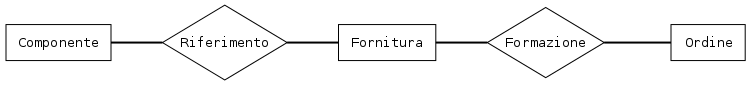
\includegraphics[width=11.5cm]{images/diagrams/componente_ordine.png}
		\end{figure}
		
		Il magazzino, nella realtà, è composto dai vari articoli acquistati che sono in attesa di essere utilizzati. La classificazione degli articoli avviene, in primo luogo per componente, in secondo luogo per fornitura d'appartenenza. Non vi è così il bisogno di registrare ogni articolo individualmente, ma basterà riferirsi alle relative forniture.
		Il \emph{Magazzino} è una composizione di \emph{Forniture} i cui articoli sono depositati in attesa di essere utilizzati.
		
		\begin{figure}[H]
			\centering
			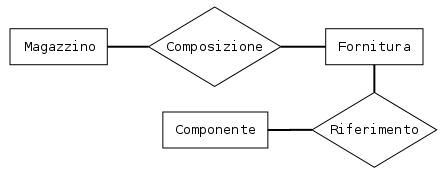
\includegraphics[width=9cm]{images/diagrams/magazzino_fornitura.png}
		\end{figure}
		
		Per identificare con precisione quali articoli sono stati utilizzati per l'esecuzione di una prestazione, sarà sufficiente riferirsi alla fornitura relativa agli stessi. Da questa si ottengono le informazioni sul componente (quindi il prezzo di vendita e il tempo di validità) e sulla data d'acquisto.
		Ad ogni utilizzo, si provvederà ad aggiornare le quantità rimanenti degli articoli delle forniture utilizzate.
		Per l'esecuzione di una \emph{Prestazione} si possono utilizzare gli articoli di più \emph{Forniture}.
		
		\begin{figure}[H]
			\centering
			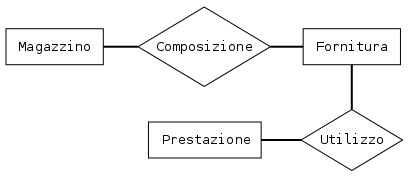
\includegraphics[width=9cm]{images/diagrams/prestazione_fornitura.png}
		\end{figure}
		
		Passiamo alla questione degli operatori. Una prestazione viene eseguita da uno o più operatori. Di ogni operatore si vuole tener traccia dei turni di lavoro effettuati.
		Alla \emph{Prestazione}, saranno associati uno o più \emph{Operatori} ad ognuno dei quali sono associati i relativi \emph{Turni} di lavoro.
		
		\begin{figure}[H]
			\centering
			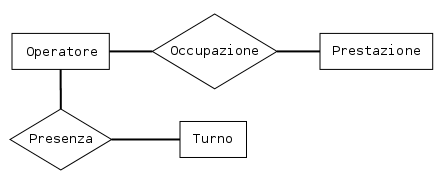
\includegraphics[width=9cm]{images/diagrams/operatore_turno_prestazione.png}
		\end{figure}
		
		Occupiamoci ora delle zone periferiche dello schema. Un preventivo viene effettuato quando un cliente richiede un intervento alla propria auto.
		Ad ogni \emph{Cliente} vengono associate una o più \emph{Autovetture}. Ogni \emph{Preventivo} si riferisce ad una specifica \emph{Autovettura}.
		
		\begin{figure}[H]
			\centering
			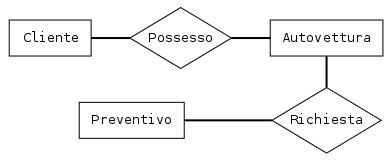
\includegraphics[width=9cm]{images/diagrams/cliente_autovettura_preventivo.png}
		\end{figure}
		
		Ogni \emph{Ordine} viene effettuato presso un \emph{Fornitore}.
		
		\begin{figure}[H]
			\centering
			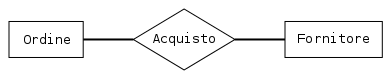
\includegraphics[width=9cm]{images/diagrams/ordine_fornitore.png}
		\end{figure}
		
		Notiamo che \emph{Cliente} rappresenta sia \emph{Privati} che \emph{Aziende} (rispettivamente, clienti non dotati di partita iva e clienti dotati di partita iva).
		
		\begin{figure}[H]
			\centering
			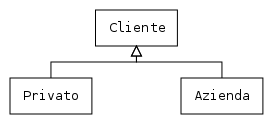
\includegraphics[width=7.5cm]{images/diagrams/cliente.png}
		\end{figure}
		
		Inoltre \emph{Clienti}, \emph{Fornitori} ed \emph{Operatori} possono essere generalizzati dall'entità \emph{Persona}.
		
		\begin{figure}[H]
			\centering
			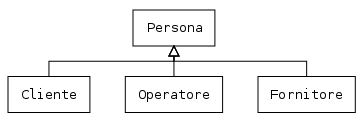
\includegraphics[width=10cm]{images/diagrams/persona.png}
		\end{figure}
		
		Ad ogni \emph{Persona} saranno associati uno o più \emph{Recapiti}.
		
		\begin{figure}[H]
			\centering
			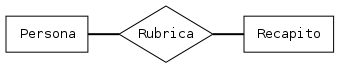
\includegraphics[width=9cm]{images/diagrams/persona_recapito.png}
		\end{figure}
		
		Possiamo concludere lo sviluppo della struttura del diagramma ER affrontando la questione delle transazioni. Avviene una \emph{Transazione} ogni volta che viene versato un acconto per un \emph{Preventivo}, ogni volta che viene saldata la \emph{Fattura} di una \emph{Prestazione}, ogni volta che viene pagato un \emph{Ordine} ed ogni volta che viene pagato lo stipendio di un \emph{Operatore}.
		
		\begin{figure}[H]
			\centering
			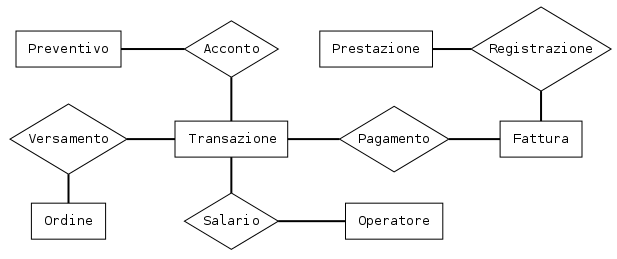
\includegraphics[width=12cm]{images/diagrams/transazione.png}
		\end{figure}
			
		Il diagramma in figura \ref{fig:scheletro_er} rappresenta lo scheletro dello schema ER.
		
		\begin{sidewaysfigure}
			\centering
			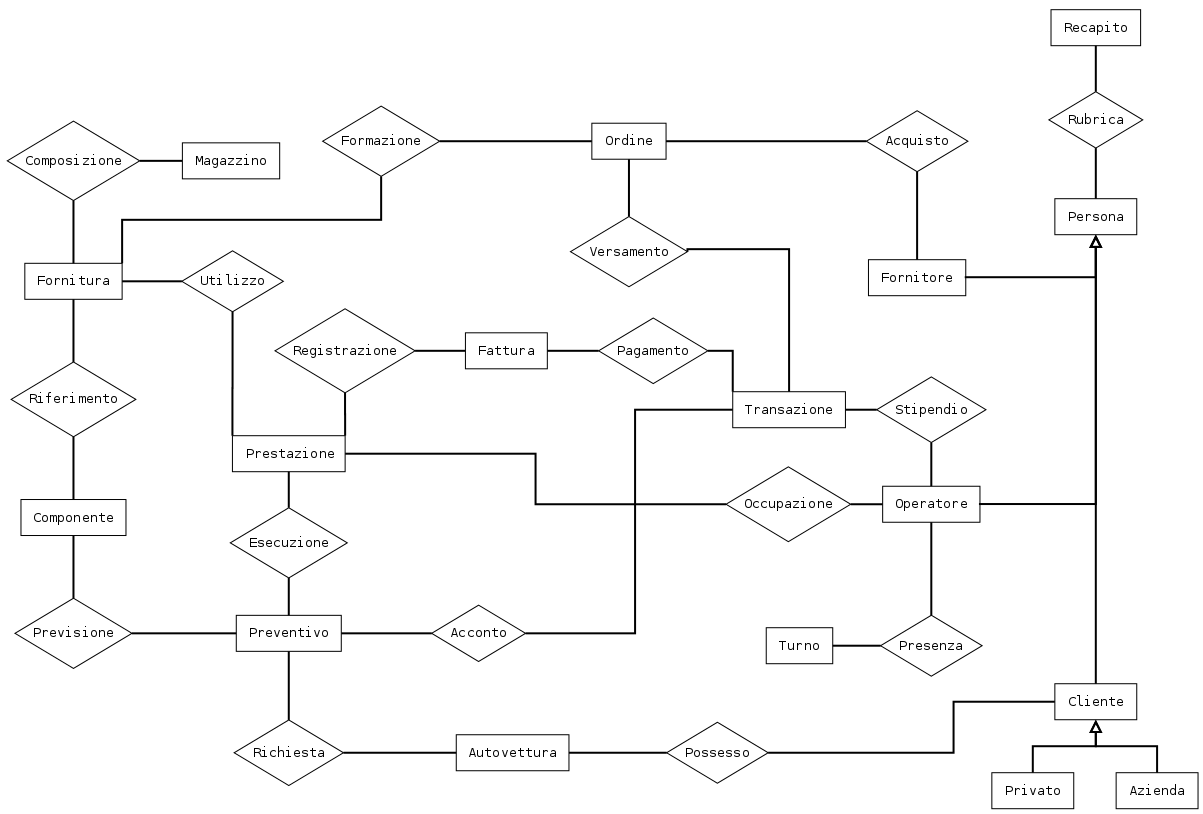
\includegraphics[width=22cm]{images/diagrams/schema.png}
			\caption{Scheletro del diagramma ER}
			\label{fig:scheletro_er}
		\end{sidewaysfigure}
	
	\subsection{Sviluppo delle Componenti dello Schema}
	
		Ottenuto lo scheletro generale del diagramma ER procediamo ad esplicitare, delle entità principali, l'insieme degli attributi che ognuna di esse possiede.
		Una volta sviluppati gli attributi delle entità principali svilupperemo le relationship che le legano, raggruppandole tra loro sulla falsariga dei modelli elaborati allo step precedente.
		
		\begin{description}
			\item[NB]
				Ogni generalizzazione effettuata è da considerarsi totale.
		\end{description}
		
		\subsubsection{Persona}
		
			In figura \ref{fig:persona} troviamo lo sviluppo degli attributi dell'entità \emph{Persona} e delle relative entità che la estendono.
			
			L'identificativo dell'entità \emph{Persona} è costituito dall'attributo "Codice Fiscale o P.Iva", capace di identificare così sia privati che aziende. Ogni \emph{Persona} è caratterizzata anche dall'attributo composto "Indirizzo", sviluppabile in "Città", "Via", "Civico", "CAP", che identifica l'indirizzo di riferimento della persona stessa.
			
			Le entità figlie di \emph{Persona} sono \emph{Fornitore}, \emph{Operatore} e \emph{Cliente}. Quest'ultimo può essere ulteriormente scomposto in altre due entità figlie \emph{Privato} e \emph{Azienda}.
			
			\emph{Privato} possiede gli attributi "Nome", "Cognome" e "Numero Documento Identità", mentre per l'entità \emph{Azienda} si è reso necessario avere solamente l'attributo "Ragione Sociale".
			
			\emph{Fornitore} è dotato degli attributi "Ragione Sociale", "IBAN", "Tempi Consegna" (numero di giorni feriali necessari in media affinchè la merce ordinata al fornitore arrivi) e "Modalità Pagamento" (specifica la modalità di pagamento tra assegno e bonifico bancario).
			
			\emph{Operatore} ha gli attributi "Nome", "Cognome", "IBAN", "Stipendio" (ammontare dello stipendio mensile, se il lavoratore ha un contratto a retribuzione fissa), "Retribuzione oraria" (se il lavoratore ha un contratto che prevede uno stipendio calcolato in base alle ore di lavoro), "Modalità Riscossione" (specifica la modalità di riscossione dello stipendio tra assegno, bonifico o contanti\footnote{Applicabile solo nel caso in cui l'ammontare del pagamento non superi l'importo massimo a norma di legge. Attualmente il limite per i pagamenti in contanti ammonta a 1000.00\EUR.}) e "Dati Anagrafici" (attributo composto da "Data di Nascita", "Comune di Nascita", "Provinicia").
						
			\begin{figure}[H]
				\centering
				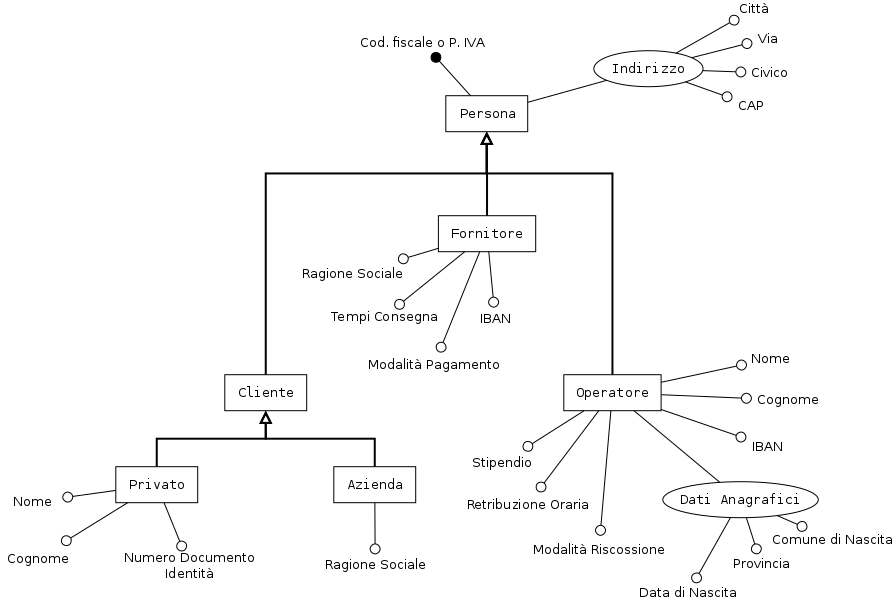
\includegraphics[width=12cm]{images/finitures/persona.png}
				\caption{Sviluppo di Persona}
				\label{fig:persona}
			\end{figure}
		
		\subsubsection{Autovettura}
			
			Continuiamo con gli attributi che caratterizzano l'entità \emph{Autovettura} (Diagramma in figura \ref{fig:autovettura})
			
			\begin{figure}[H]
				\centering
				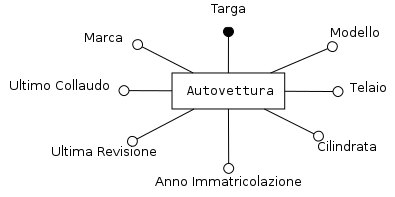
\includegraphics[width=9cm]{images/finitures/autovettura.png}
				\caption{Sviluppo dell'entità Autovettura}
				\label{fig:autovettura}
			\end{figure}
			
			\emph{Autovettura} comprende gli attributi "Targa", "Marca", "Modello", "Telaio" (numero di serie del telaio che identifica univocamente un veicolo che viene inciso sul telaio del veicolo e viene indicato nel libretto di circolazione), "Ultima Revisione" e "Ultimo Collaudo" (rispettivamente le date in cui è stata effettuata la revisione dell'auto e il collaudo di un eventuale impianto di alimentazione differente da quello di fabbricazione), "Anno di Immatricolazione", "Cilindrata".
		
			Si è scelto l'attrubuto "Targa" come chiave primaria dell'entità piuttosto che l'attributo "Telaio" nonostante anche quest'ultimo identifichi univocamente l'autovettura. Riteniamo che sia più agevole identificare un'autovettura attraverso la targa poichè tale informazione è più facilmente reperibile rispetto al seriale del telaio.
			
		\subsubsection{Preventivo}
		
			In figura \ref{fig:preventivo}, il diagramma espone gli attributi dell'entità \emph{Preventivo}.
			
			\emph{Preventivo} è costituito dagli attributi "Codice" (identificativo numerico interno all'azienda del preventivo fornito), "Data Emissione", "Tempo Stimato" (ovvero la stima del numero di giorni necessari all'esecuzione del lavoro), "Data Inizio" (data in cui il lavoro è stato pianificato per essere eseguito), "Categoria" (riparazione, installazione di un impianto a metano, installazione di un impianto a gpl, collaudo o revisione), "Sistema Alimentazione" (attributo necessario per le installazioni di nuovi impianti, necessari a specificare il sistema di alimentazione tra sistema a iniezione e sistema ad aspirazione), "Sintomi" (ovvero una breve descrizione del malfunzionamento riscontrato, nel caso in cui si tratti di una riparazione), "Costo Servizi" (composizione della stima dei costi dei servizi aggiuntivi e della manodopera).
			
			\begin{figure}[H]
				\centering
				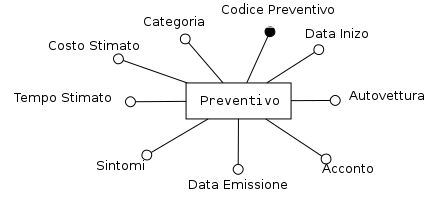
\includegraphics[width=12cm]{images/finitures/preventivo.png}
				\caption{Sviluppo dell'entità Preventivo}
				\label{fig:preventivo}
			\end{figure}
			
		\subsubsection{Prestazione}
			
			Gli attributi dell'entità \emph{Prestazione} vengono esplicitati dal diagramma in figura \ref{fig:prestazione}.
			
			\emph{Prestazione} è composta dagli attributi "Preventivo" (codice identificativo del preventivo di riferimento), "Tempi Esecuzione" (giorni necessari effettivamente all'esecuzione del lavoro preventivato), "Malfunzionamento" (descrizione breve della natura e dell'origine del malfunzionamento riscontrato), "Procedimento" (descrizione concisa ed essenziale del procedimento utilizzato per eliminare i malfunzionamenti), "Costo Servizi" (attributo composto dal costo \emph{effettivo} dei servizi aggiuntivi e della manodopera).
		
			Dovendo tener traccia del preventivo di riferimento a fronte di una prestazione fornita, abbiamo scelto l'attributo \emph{Preventivo} come chiave primaria, dal momento che non vi possono essere più prestazioni a fronte dello stesso preventivo.
		
			\begin{figure}[H]
				\centering
				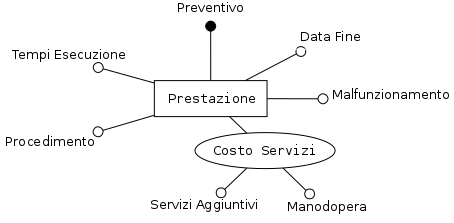
\includegraphics[width=9cm]{images/finitures/prestazione.png}
				\caption{Sviluppo dell'entità Prestazione}
				\label{fig:prestazione}
			\end{figure}
		
		\subsubsection{Componente}
			
			Nel diagramma in figura \ref{fig:componente} troviamo l'entità \emph{Componente} ed i relativi attributi.
			
			L'entità \emph{Componente} comprende gli attributi "Codice" (identificativo numerico interno del componente), "Nome", "Validità" (giorni dalla data di acquisto dopo i quali il componente diventa inutilizzabile), "Quantità Minima" (quantitativo minimo da avere sempre in magazzino), "Prezzo Vendita" (prezzo unitario al quale il componente viene venduto). 
			
			\begin{figure}[H]
				\centering
				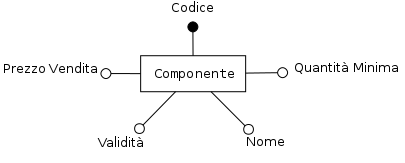
\includegraphics[width=9cm]{images/finitures/componente.png}
				\caption{Sviluppo di Componente}
				\label{fig:componente}
			\end{figure}
		
		\subsubsection{Fattura}
		
			Nel diagramma in figura \ref{fig:fattura}, l'entità \emph{Fattura} ed i suoi attributi.
		
			\begin{figure}[H]
				\centering
				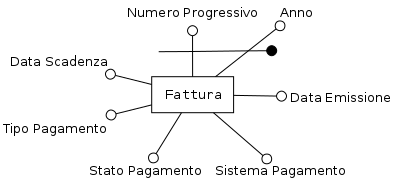
\includegraphics[width=9cm]{images/finitures/fattura.png}
				\caption{Sviluppo di Transazione}
				\label{fig:fattura}
			\end{figure}
			
			\emph{Fattura} è composta dagli attributi "Numero Progressivo" e "Anno" (coppia di attributi identificatori, derivano direttamente dalla struttura reale delle fatture), "Totale" (descrive il prezzo totale della prestazione, è composto da "Imposte", "Imponibile", "Sconto"\footnote{Quantità espressa in percentuale. Consultare \ref{rv:sconto}. }, "Incentivi"), "Data Emissione", "Sistema Pagamento" (specifica uno dei due sistemi di pagamento accettati: rimessa diretta e rimessa differita), "Tipo Pagamento" (metodologie di pagamento accettate: bonifico, contanti o assegno), "Stato Pagamento" (attributo booleano che permette di distinguere le fatture saldate da quelle non ancora pagate), "Data Scadenza" (data entro la quale la fattura deve essere saldata).
		
		\subsubsection{Transazione}
			
			Il diagramma in figura \ref{fig:transazione} raffigura lo sviluppo degli attributi dell'entità \emph{Transazione}.
			
			L'entità \emph{Transazione} è semplicemente composta dagli attributi "Codice", "Quota" (ammontare della transazione di denaro: quantità positiva per le transazioni entranti, negativa per quelle uscenti), "Data".
						
			\begin{figure}[H]
				\centering
				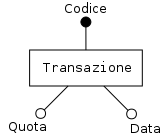
\includegraphics[width=4.5cm]{images/finitures/transazione.png}
				\caption{Sviluppo di Transazione}
				\label{fig:transazione}
			\end{figure}
		
		\subsubsection{Raffinamenti Successivi}
			
			Esplicitati gli attributi delle principali entità, procediamo a legarle tra loro sviluppando le relationship ed alcune entità minori.
			
			Ripercorrendo i passi dello sviluppo dello scheletro del diagramma ER, partiamo dalle relationship che legano le entità \emph{Cliente}, \emph{Autovettura}, \emph{Preventivo} (diagramma in figura \ref{fig:cliente_autovettura_preventivo}).		
		
			\begin{figure}
				\centering
				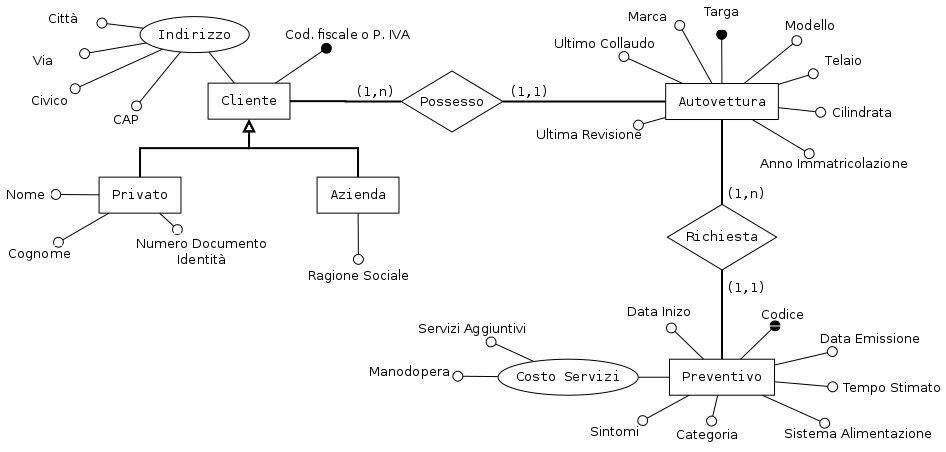
\includegraphics[width=13cm]{images/finitures/cliente_autovettura_preventivo.png}
				\caption{Sviluppo delle relationship che legano Cliente, Autovettura e Preventivo}
				\label{fig:cliente_autovettura_preventivo}
			\end{figure}
			
			Chiaramente ad ogni cliente registrato, saranno associate una o più autovetture di sua propiertà. Ad ogni autovettura saranno associati uno o più preventivi di interventi riferiti all'autovettura stessa (Diagramma in figura \ref{fig:cliente_autovettura_preventivo}).
			
			Se l'intervento preventivato viene realizzato, al preventivo sarà associata una ed una sola prestazione. La stipulazione del preventivo non è vincolante nei confronti del cliente, quindi non è vero che ad ogni preventivo corrisponde una prestazione (Diagramma in figura \ref{fig:preventivo_prestazione}).
			
			\begin{figure}[H]
				\centering
				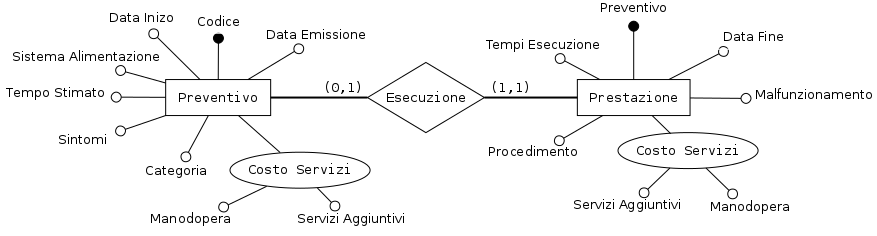
\includegraphics[width=13cm]{images/finitures/preventivo_prestazione.png}
				\caption{Sviluppo della relationship che lega Preventivo e Prestazione}
				\label{fig:preventivo_prestazione}
			\end{figure}
			
			I componenti previsti nelle riparazioni vengono descritti tramite la relazione \emph{Previsione} che lega le entità \emph{Componente} e \emph{Preventivo}. In ogni preventivo si può prevedere di utilizzare nessuno, uno o più componenti. L'utilizzo di uno stesso componente può essere previsto - ovviamente - nella formulazione di più preventivi.
			Si consulti il diagramma in figura \ref{fig:preventivo_componente}.
			
			\begin{figure}[H]
				\centering
				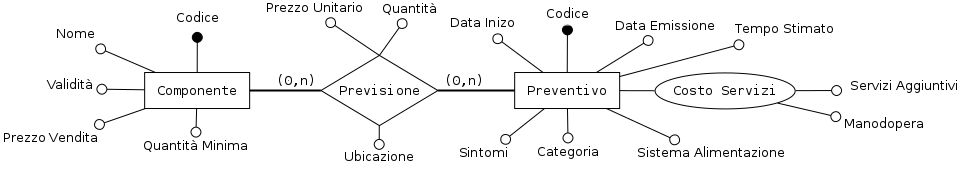
\includegraphics[width=13cm]{images/finitures/preventivo_componente.png}
				\caption{Sviluppo di Preventivo e Componente}
				\label{fig:preventivo_componente}
			\end{figure}
			
			L'attributo "Ubicazione" della relazione \emph{Previsione} rappresenta l'ubicazione dei componenti utilizzati nelle installazioni di nuovi impianti (si consultino anche le specifiche riguardanti i preventivi alla sottosezione "Frasi relative ai Preventivi" \ref{sec:frasi_preventivi}).
			L'attributo "Prezzo Unitario" della relazione \emph{Previsione} si rivela necessario, in quanto il prezzo di vendita dei singoli componenti è soggetto a variazioni nel tempo.
			
			Per la registrazione degli articoli acquistati sono state introdotte in fase di sviluppo dello scheletro dello schema ER le entità \emph{Ordine} e \emph{Fornitura}. Tali entità, prese singolarmente, sono poco significative, essendo fortemente legate tra di loro (si faccia riferimento al diagramma in figura \ref{fig:fornitore_ordine_fornitura_componente}).
			
			I contratti di acquisto con i fornitori vengono modellati dall'entità \emph{Ordine}. Naturalmente presso lo stesso fornitore si possono effettuare più ordini, ma un ordine si riferisce ad un singolo fornitore. \emph{Ordine} e \emph{Fornitore} sono legati dalla relationship \emph{Acquisto}.
			
			\begin{figure}[H]
				\centering
				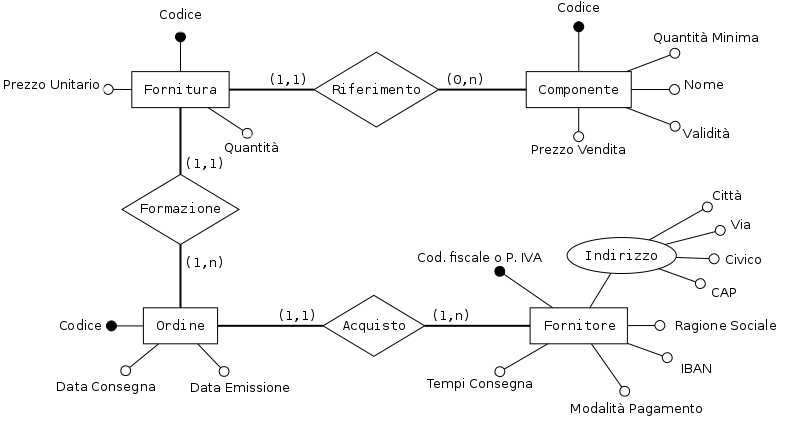
\includegraphics[width=13cm]{images/finitures/fornitore_ordine_fornitura_componente}
				\caption{Sviluppo delle relazioni che legano il Fornitore, l'Ordine d'acquisto, le Forniture e i Componenti}
				\label{fig:fornitore_ordine_fornitura_componente}
			\end{figure}
			
			Ogni ordine è composto da una o più forniture, le quali, a loro volta, sono composte da uno o più articoli dello stesso componente. Ad ogni istanza dell'entità \emph{Fornitura} si associa - tramite la relationship \emph{Riferimento} - una ed una sola istanza dell'entità \emph{Componente}. Di contro, lo stesso componente può essere acquistato in diverse forniture.
			Quindi ogni istanza di \emph{Fornitura} sarà associata ad una ed una sola istanza di \emph{Ordine} tramite la relationship \emph{Formazione}. Un ordine vedrà associate a sè una o più forniture.
			
			\begin{figure}
				\centering
				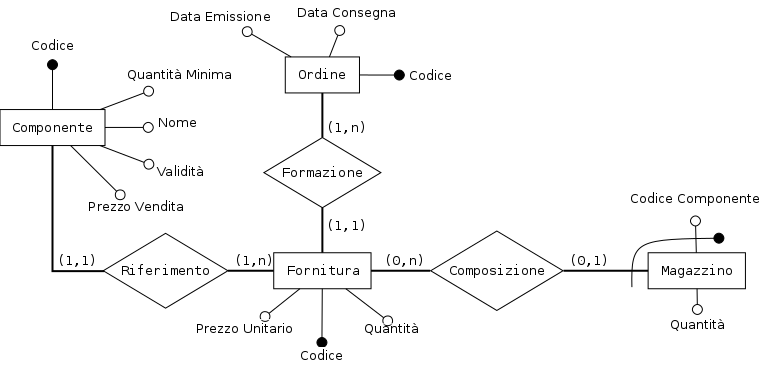
\includegraphics[width=13cm]{images/finitures/componente_fornitura_ordine_magazzino.png}
				\caption{Introduzione del Magazzino}
				\label{fig:componente_fornitura_ordine_magazzino}
			\end{figure}
			
			Un'ulteriore entità da aggiungere a questo gruppo è quella del magazzino. Abbiamo definito \emph{Magazzino} come una raccolta di forniture attive, cioè di forniture i quali articoli sono ancora presenti nel magazzino fisico, pronti per essere utilizzati. Legando \emph{Magazzino} con \emph{Fornitura} si modella tale associazione. La relationship \emph{Composizione} associa ad ogni istanza di \emph{Magazzino} una ed una sola istanza di \emph{Fornitura}.
			Fare riferimento al diagramma in figura \ref{fig:componente_fornitura_ordine_magazzino}.
			
			Da notare che l'attributo "Quantità" dell'entità \emph{Magazzino} descrive il numero di articoli di uno specifico componente, acquistati in una certa fornitura, ancora disponibili in magazzino.
			
			All'esecuzione di una prestazione, come da specifiche, è necessario specificare il tipo e la quantità di articoli utilizzati. La prima soluzione che ci è sembrata valida è stata quella di associare, ad ogni istanza dell'entità \emph{Prestazione} le istanze interessate dell'entità \emph{Componente} attraverso la relationship \emph{Utilizzo}. Tale relationship avrebbe avuto l'attributo "Quantità", necessario per specificare la quantità degli articoli utilizzati per ogni componente.
			
			Tuttavia, tale design si è rivelato non adeguato a soddisfare tutte le specifiche. Il problema più evidente risiedeva nel fatto che, essendo le istanze dell'entità \emph{Componente} composte da informazioni descrittive, pressocchè invarianti (eccezion fatta per quanto riguarda il "Prezzo di Vendita"), non vi è il modo per risalire al preciso articolo fisico utilizzato nella riparazione\footnote{Non potendo risalire al preciso articolo utilizzato, non si ha a disposizione la data di acquisto, quindi viene meno la realizzabilità del meccanismo che permette di utilizzare per primi gli articoli dei componenti la cui data di scadenza è più vicina di altri.}.
			
			All'entità \emph{Prestazione} vengono quindi associate zero, una o più istanze dell'entità \emph{Fornitura}, avendo così a disposizione sia le informazioni che descrivono genericamente il componente, sia quelle che caratterizzano con precisione l'articolo utilizzato nella prestazione. 

			\begin{figure}
				\centering
				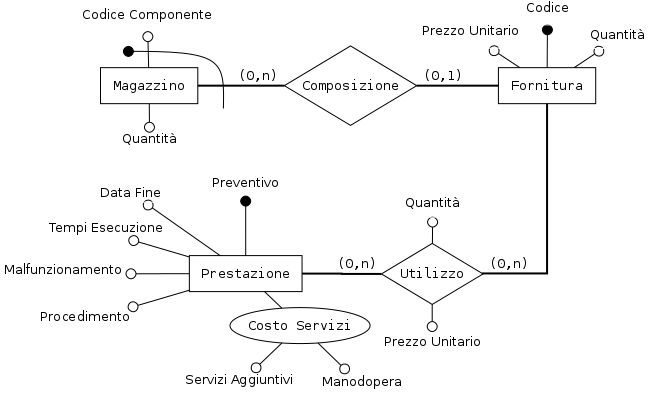
\includegraphics[width=11.5cm]{images/finitures/prestazione_fornitura.png}
				\caption{Utilizzo di componenti un una prestazione}
				\label{fig:ordine_fornitore}
			\end{figure}
			
			L'attributo "Quantità" della relationship \emph{Utilizzo} non necessita di ulteriori spiegazioni, mentre l'attributo "Prezzo Unitario" si rende necessario, in quanto il prezzo di vendita di un componente, ragionevolmente, varia nel tempo.
			
			Ad esecuzione ultimata di una prestazione avviene la registrazione della fattura. Ad ogni istanza dell'entità \emph{Prestazione} sarà associata, tramite la relationship \emph{Registrazione} obbligatoriamente una ed una sola istanza dell'entità \emph{Fattura}. 		
			
			Le istanze dell'entità \emph{Fattura} vengono identificate dalla coppia di attributi "Numero Progressivo" ed "Anno", così come avviene nella realtà di interesse\footnote{Le fatture vengono identificate dall'anno di emissione e dal numero progressivo. Ogni anno tale numero viene azzerato.}.
			
			\begin{figure}
				\centering
				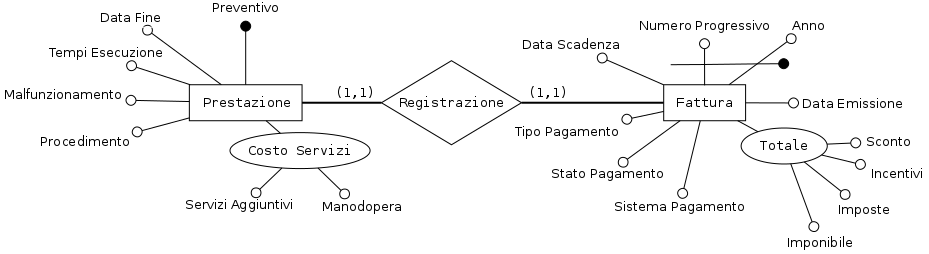
\includegraphics[width=11.5cm]{images/finitures/prestazione_fattura.png}
				\caption{Sviluppo della relationship tra Prestazione e Fattura}
				\label{fig:prestazione_fattura}
			\end{figure}
			
			Gli sviluppi dei diagrammi introdotti fin'ora permettono di affrontare il legame di \emph{Transazione} con le altre entità. A quest'ultima si possono associare istanze di tutte le entità che modellano dati di porzioni di processo che prevedono il verificarsi di transazioni monetarie. Alla stipulazione di un preventivo può essere richiesto il versamento di un acconto, alla consegna gli ordine sarà necessario effettuare una versamento al fornitore, mensilmente bisognerà registrare gli stipendi versati agli operatori e quando una fattura viene saldata bisognerà registrare tale transazione di denaro.
			
			\begin{figure}
				\centering
				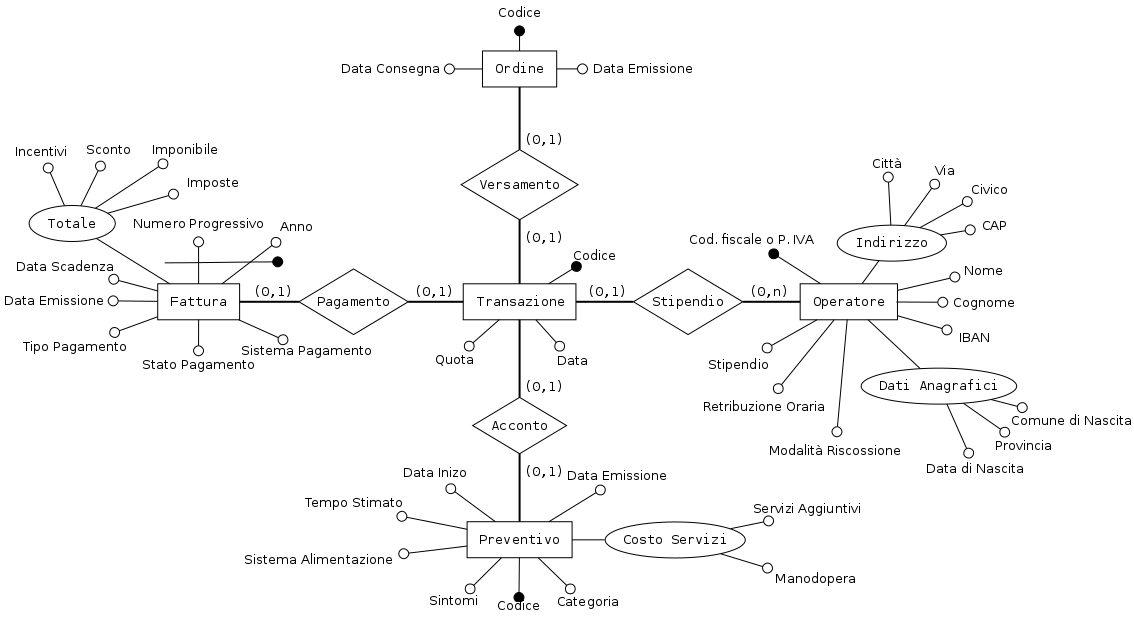
\includegraphics[width=13cm]{images/finitures/transazione_fattura_preventivo_operatore_ordine.png}
				\caption{Sviluppo delle relationship con cui Transazione si lega alle altre entità}
				\label{fig:transazione_fattura_preventivo_operatore_ordine}
			\end{figure}
			
			Nel diagramma in figura \ref{fig:transazione_fattura_preventivo_operatore_ordine} vi è la rappresentazione di come le entità \emph{Preventivo}, \emph{Ordine}, \emph{Operatore}, \emph{Fattura} vengono associate a \emph{Transazione}.
			
			Esaminiamo le ultime componenti del diagramma ER che non sono state ancora analizzate.
			
			In figura \ref{fig:operatore_prestazione} il diagramma descrive la relationship \emph{Occupazione} che associa le istanze di \emph{Prestazione} a quelle di \emph{Operatore}. Ad ogni istanza di \emph{Prestazione} infatti devono essere associate una o più instanze di \emph{Operatore}, in modo da tener traccia dei dipendenti che sono stati impiegati nell'esecuzione della prestazione ad un'autovettura. Ovviamente la stessa istanza di \emph{Operatore} può essere associata a più istanze di \emph{Prestazione}.
			
			\begin{figure}
				\centering
				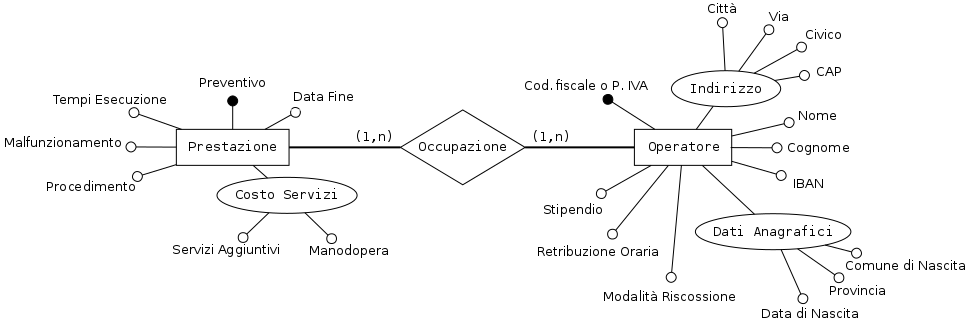
\includegraphics[width=11.5cm]{images/finitures/operatore_prestazione.png}
				\caption{Sviluppo della relationship tra Prestazione e Operatore}
				\label{fig:operatore_prestazione}
			\end{figure}
			
			Riguardo gli operatori è necessario, come da specifiche, registrarne le presenze e gli orari di lavoro. L'entità \emph{Turno}, legata ad \emph{Operatore} tramite la relationship \emph{Presenza} (diagramma in figura \ref{fig:operatore_turno}), assolve tale funzione.
			
			\begin{figure}
				\centering
				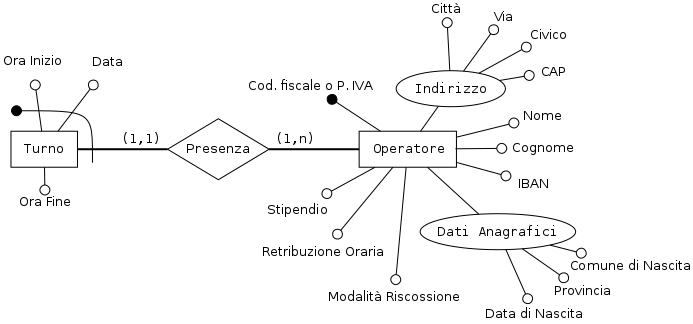
\includegraphics[width=11.5cm]{images/finitures/operatore_turno.png}
				\caption{Turni degli Operatori}
				\label{fig:operatore_turno}
			\end{figure}
			
			L'ultimo punto da sviluppare consiste nella gestione dei recapiti, di qualunque natura essi siano. L'entità \emph{Recapito} è costituita dagli attributi "Codice" (che ne è anche la chiave primaria), "Recapito" e "Tipo" (consultare le Regole Aziendali alla sezione \ref{sec:business_rules} per i valori che tale attributo può assumere).

			Ad ogni istanza di \emph{Persona} devono essere associati una o più istanze di \emph{Recapito}. 
			Più istanze di \emph{Persona} possono essere associate alla stessa istanza di \emph{Recapito}: si tratta di un caso particolare, legato soprattutto all'entità \emph{Cliente}, figlia di \emph{Persona}.
			Ad esempio due clienti dello stesso nucleo familiare condividono lo stesso numero di telefono, da qui la necessità di non vincolare le partecipazioni delle istanze di \emph{Recapito} nella relationship \emph{Rubrica} ad una ed una sola.
			
			\begin{figure}[H]
				\centering
				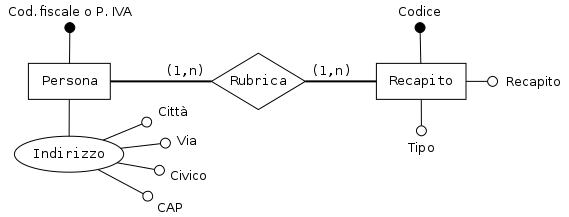
\includegraphics[width=11.5cm]{images/finitures/persona_rubrica.png}
				\caption{Recapiti associati ad una Persona}
				\label{fig:persona_recapito}
			\end{figure}
	
	% Diagramma definitivo
	\subsection{Diagramma Entity-Relationship}
		
		L'intero diagramma ER si può trovare in figura \ref{fig:er}.
			
		\begin{sidewaysfigure}
			\centering
			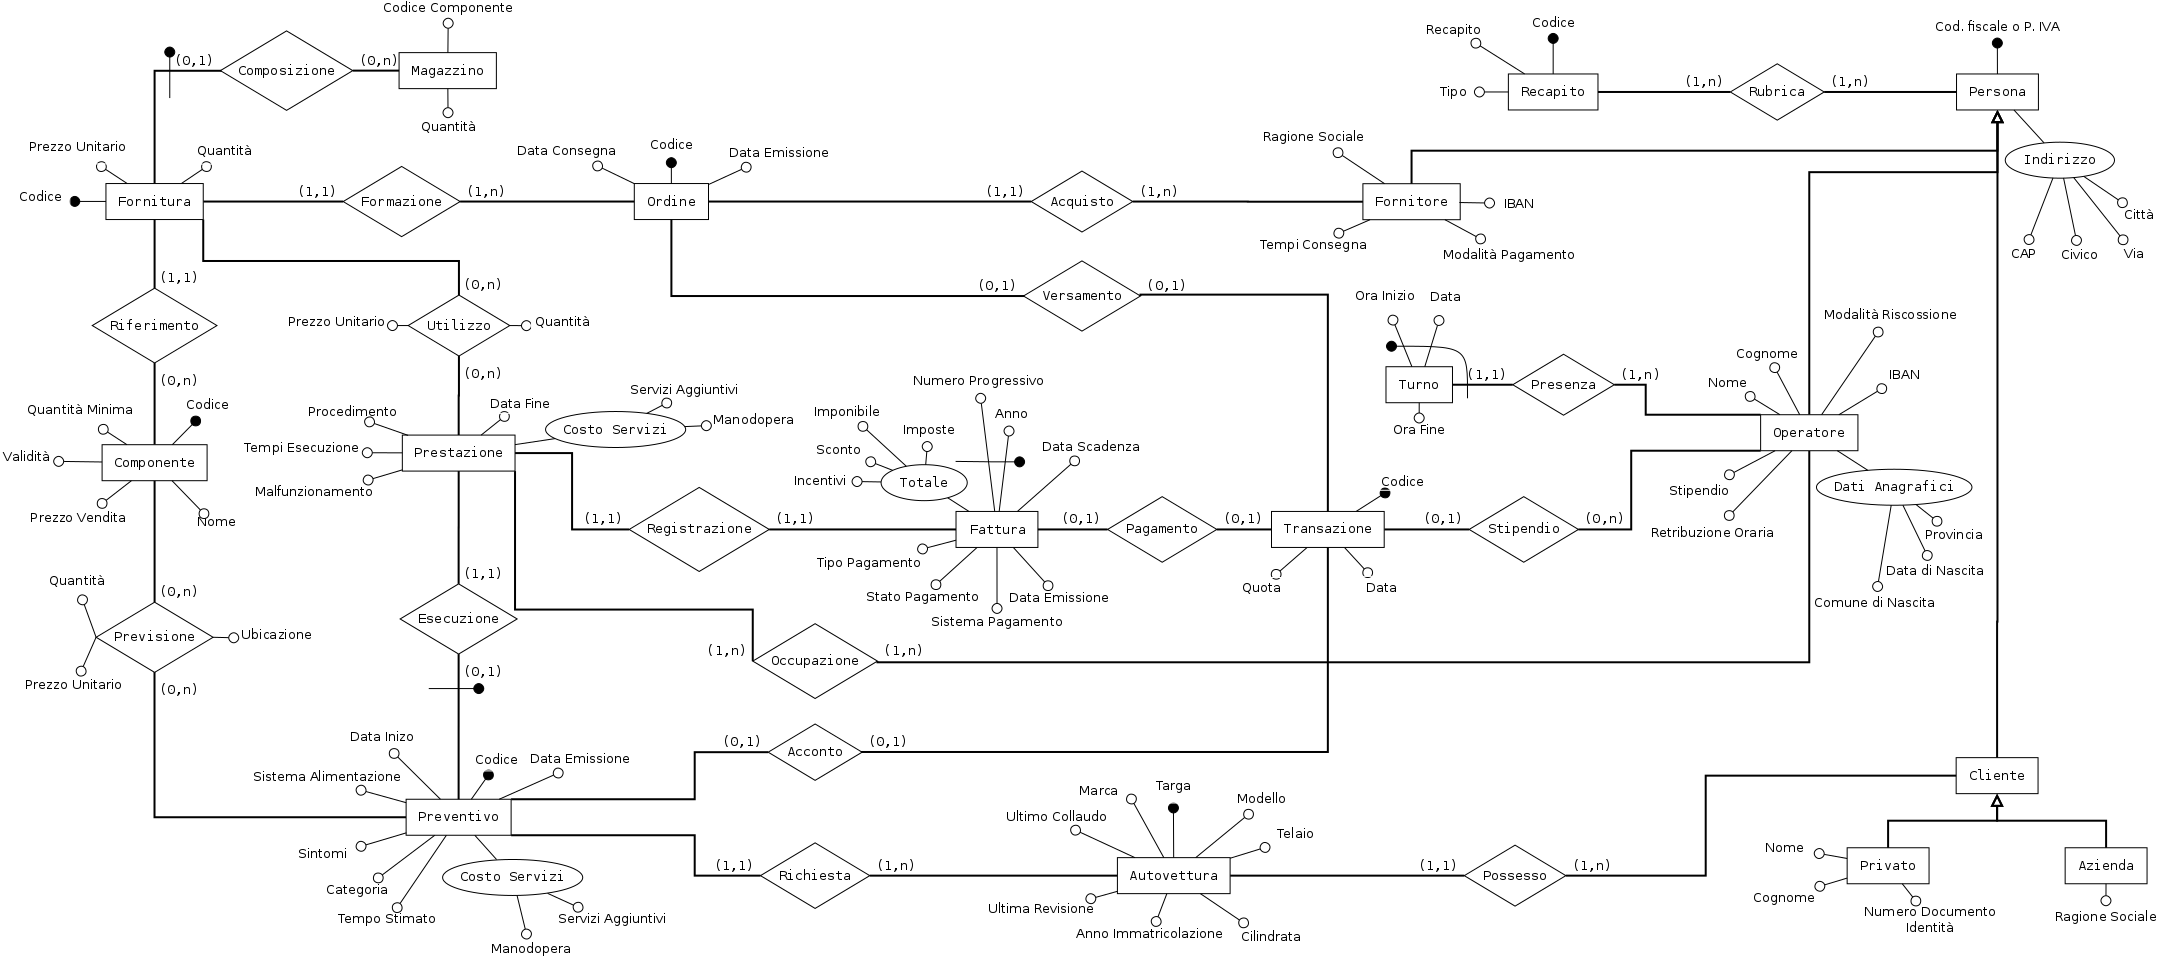
\includegraphics[width=22cm]{images/finitures/schema.png}
			\caption{Scheletro del diagramma ER}
			\label{fig:er}
		\end{sidewaysfigure}

		\newpage

	\subsection{Analisi Qualitativa dello Schema ER}
		
		Effettuiamo una breve analisi in termini qualitativi del diagramma ER sviluppato.
		
		\begin{description}
			\item[Correttezza] Il diagramma sviluppato fa un uso sintatticamente e semanticamente corretto dei costrutti disponibili del modello Entità-Relazione.
			\item[Completezza] Confrontando il diagramma risultante con le specifiche che abbiamo individuato nell'Analisi dei Requisiti (sezione \ref{sec:req_analysis}), reputiamo che quest'ultime siano soddisfatte.
			\item[Leggibilità] Abbiamo strutturato graficamente il diagramma in modo da favorirne il più possibile la leggibilità. In particolare ci siamo focalizzati sul minimizzare il numero di intersezioni tra gli archi che collegano entità e relationship, non riuscendo tuttavia ad evitarle del tutto.
			\item[Minimalità] Il diagramma non è del tutto privo di parti ridondanti. Gli attributi \emph{Imponibile} ed \emph{Imposte} relative all'entità \emph{Fattura} introductono ridondanza nella rappresentazione dell'imformazione (consultare per maggiori informazioni le Regole di Derivazione \ref{rd:imponibile} e \ref{rd:imposte}). Valuteremo nelle prossime fasi progettuali se eliminare o meno tale ridondanza.
		\end{description}
		
		Il diagramma, nonostante l'assenza di minimalità, risulta valido, adeguato per procedere ai successivi passi progettuali.
	
	% Sezione documentativa della progettazione concettuale
	\subsection{Dizionario dei Dati}
	\label{sec:data_dict}
		
		\subsubsection{Entità}
		\label{sec:entities}
			
			\begin{description}
				\item[NB] Esplicitiamo gli attributi composti elencando tra le parentesi quadre gli attributi semplici di cui sono costituiti.
			\end{description}
	
			{\small
			\begin{longtable}{| p{2cm} | p{4cm} | p{4cm} | p{2cm} |}
				
				\hline
				\textbf{Nome} & 
				\textbf{Descrizione} & 
				\textbf{Attributi} & 
				\textbf{Identificatore} \\ 
				\hline
				
				\endfirsthead
				
				\hline
				\textbf{Nome} & 
				\textbf{Descrizione} & 
				\textbf{Attributi} & 
				\textbf{Identificatore} \\ 
				\hline
				
				\endhead
				
				Persona &
				Soggetto generico che intrattenga rapporti di ogni tipo con l'azienda. &
				Codice Fiscale o P.IVA (Stringa), Indirizzo [Città (Stringa), Via (Stringa), Civico (Numerico), CAP (Numerico)] &
				Codice Fiscale o P.IVA (Stringa)
				\\ \hline

				Cliente &
				Soggetto che necessita di un servizio da parte dell'azienda. &
				// &
				//
				\\ \hline

				Privato &
				Cliente non dotato di partita IVA. &
				Attributi di Persona, Nome (Stringa), Cognome (Stringa), Numero Documento Identità (Stringa) &
				//
				\\ \hline

				Azienda &
				Cliente dotato di partita IVA. &
				Attributi di Persona, Ragione Sociale (Stringa) &
				//
				\\ \hline

				Fornitore &
				Azienda che abbia fornito all’officina qualsiasi tipo di componente necessario. &
				Attributi di Persona, Ragione Sociale (Stringa), Tempi Consegna (Numerico), Modalità Pagamento (Stringa), IBAN (Stringa) &
				//
				\\ \hline

				Operatore &
				Lavoratore dell'azienda. &
				Attributi di Persona, Nome (Stringa), Cognome (Stringa), IBAN (Stringa), Stipendio (Numerico), Retribuzione Oraria (Numerico), Modalità Riscossione (Stringa), Dati Anagrafici [Comune Nascita (Stringa), Provincia (Stringa), Data Nascita (Data)] &
				//
				\\ \hline

				Autovettura &
				Automobile di un cliente che debba subire o abbia già subito un intervento da parte dei lavoratori dell’azienda. &
				Targa (Stringa), Modello (Stringa), Telaio (Stringa), Cilindrata (Numerico), Anno Immatricolazione (Numerico), Ultima Revisione (Data), Ultimo Collaudo (Data), Marca (Stringa) &
				Targa (Stringa)
				\\ \hline

				Preventivo &
				Stima dei costi, dei tempi e dei componenti necessari relativi all’esecuzione di un intervento su un’autovettura. &
				Codice (Numerico), Data Emissione (Data), Data Inizio (Data), Categoria (Stringa), Costo Servizi [Servizi Aggiuntivi (Numerico), Manodopera (Numerico)], Tempo Stimato (Numerico), Sintomi (Stringa), Sistema Alimentazione (Stringa) &
				Codice (Numerico)
				\\ \hline

				Componente &
				Qualsiasi oggetto fisico necessario alla corretta esecuzione di una riparazione o di una installazione di un impianto su di un’autovettura. &
				Codice (Numerico), Quantità Minima (Numerico), Prezzo Vendita (Numerico), Validità (Numerico), Nome (Stringa) &
				Codice (Numerico)
				\\ \hline

				Fornitura &
				Insieme dello stesso componente inviata da un fornitore. &
				Codice (Numerico), Prezzo Unitario (Numerico), Quantità (Numerico) &
				Codice (Numerico)
				\\ \hline

				Ordine &
				Insieme di forniture inviate nello stesso momento e dallo stesso ordine. &
				Codice (Numerico), Data Consegna (Data), Data Emissione (Data) &
				Codice (Numerico)
				\\ \hline
				
				Magazzino &
				Insieme di tutte le forniture non esaurite. &
				Codice Componente (Numerico), Quantità (Numerico) &
				Codice (di \emph{Fornitura})
				\\ \hline

				Prestazione &
				Attività eseguita dagli operatori dell’officina su di un’autovettura. &
				Codice (di \emph{Preventivo}), Tempi Esecuzione (Numerico), Data Fine (Data), Costo Servizi [Manodopera (Numerico), Servizi Aggiuntivi (Numerico)], Malfunzionamento (Stringa), Procedimento (Stringa) &
				Codice (di \emph{Preventivo})
				\\ \hline

				Turno &
				Arco temporale specifico in cui gli operatori compiono le loro mansioni. &
				Ora Inizio (Numerico), Ora fine (Numerico), Data (Data) &
				Ora Inizio (Numerico), Data (Data), Codice Fiscale o P.IVA (di \emph{Operatore})
				\\ \hline

				Transazione &
				Flusso di denaro uscente o entrante nella cassa dell’attività. &
				Codice (Numerico), Quota (Numerico), Data (Data) &
				Codice (Numerico)
				\\ \hline

				Fattura &
				Documento fiscale relativo ad un pagamento da ricevere da parte di un cliente. &
				Numero Progressivo (Numerico), Anno (Numerico), Data Emissione (Data), Totale [Imponibile (Numerico), Imposte (Numerico), Sconto (Numerico), Incentivi (Numerico)], Sistema Pagamento (Stringa), Tipo Pagamento (Stringa), Stato Pagamento (Stringa), Data Scadenza (Data) &
				Numero Progressivo (Numerico), Anno (Numerico)
				\\ \hline
				
				Recapito &
				Numero telefonico, indirizzo email o sito web. Qualsiasi recapito telematico utile a contattare una Persona. &
				Codice (Numerico), Recapito (Stringa), Tipo(Stringa) &
				Codice (Numerico)
				\\ \hline
				
			\end{longtable}
			}

		\subsubsection{Relazioni}
		\label{sec:relationships}
			{\small
			\begin{longtable}{| p{2cm} | p{4cm} | p{3cm} | p{3cm} |}
				
				\hline
				\textbf{Nome} & 
				\textbf{Descrizione} & 
				\textbf{Entità Coinvolte} & 
				\textbf{Attributi} \\ 
				\hline
				
				\endfirsthead
				
				\hline
				\textbf{Nome} & 
				\textbf{Descrizione} & 
				\textbf{Entità Coinvolte} & 
				\textbf{Attributi} \\ 
				\hline
				
				\endhead
				
				Esecuzione &
				Associa ad un Preventivo una Prestazione &
				Preventivo (0, 1), Prestazione (1, 1) &

				\\ \hline

				Previsione &
				Associa i Componenti previsti in fase di stipulazione dei Preventivi &
				Componente (0, N), Preventivo (0, N) &
				Quantità (Numerico) indica la quantità del componente che si prevede di utilizzare; Ubicazione (Stringa) indica la posizione del componente preventivato nell'autovettura; Prezzo Unitario (Numerico) indica il prezzo attuale del componente.
				\\ \hline

				Formazione &
				Associa le forniture che compongono un ordine &
				Fornitura (1, 1), Ordine (1, N) &

				\\ \hline

				Composizione &
				Associa le Forniture che compongono il Magazzino aziendale &
				Magazzino (0, N), Fornitura (0, 1) &

				\\ \hline

				Riferimento &
				Associa i Componenti che descrivono una Fornitura &
				Componente (0, N), Fornitura (1, 1) &

				\\ \hline

				Utilizzo &
				Associa i Componenti relativi ad un Fornitura effettivamente usati per compiere una prestazione &
				Fornitura (0, N), Prestazione (0, N) &
				Quantità (Numerico) indica la quantità del componente che si è utilizzata; Prezzo Unitario (Numerico) indica il prezzo di vendita del componente al momento dell'utilizzo.
				\\ \hline

				Occupazione &
				Associa un Operatore ad una Prestazione da svolgere &
				Operatore (1, N), Prestazione (1, N) &
				\\ \hline

				Presenza &
				Associa un Operatore con il Turno di lavoro effettuato &
				Operatore (1, N), Turno (1, 1) &
				\\ \hline

				Possesso &
				Associa una o più Autovetture ad un Cliente &
				Cliente (1, N), Autovettura (1, 1) &
				\\ \hline

				Richiesta &
				Associa un Preventivo riferito ad una Prestazione da richiedere su una determinata Autovettura &
				Autovettura (1, N), Preventivo (1, 1) &
				\\ \hline

				Acquisto &
				Associa un Ordine effettuato da un determinato Fornitore &
				Ordine (1, 1), Fornitore (1, N) &
				\\ \hline

				Rubrica &
				Associa una generica Persona ai sui Recapiti &
				Persona (1, N), Recapito (1, N) &
				\\ \hline

				Acconto &
				Associa un Preventivo e la Transazione monetaria che un cliente può lasciare &
				Preventivo (0, 1), Transazione (0, 1) &
				\\ \hline

				Registrazione &
				Associa una Prestazione ad una Fattura &
				Prestazione (1, 1), Fattura (1, 1) &
				\\ \hline

				Pagamento &
				Associa il manifestarsi della Transazione di pagamento riferita ad una Fattura &
				Fattura (0, 1), Transazione (0, 1) &
				\\ \hline

				Versamento &
				Associa la Transazione monetaria relativa ad un Ordine &
				Ordine (0, 1), Transazione (0, 1) &
				\\ \hline

				Stipendio &
				Associa la Transazione relativa al pagamento dello stipendio di un Operatore &
				Operatore (0, N), Transazione (0, 1) &
				\\ \hline

			\end{longtable}
			}
		
	
	\subsection{Regole Aziendali}
	\label{sec:business_rules}
	
		\subsubsection{Regole di Vincolo}
		
			\setenumerate[1]{label=RV\arabic*}
			\begin{enumerate}
				
				% Si possono implementare le reference agli elementi delle liste
				% impostando come sempre \label{itm:nome} e richiamandola con 
				% \ref{itm:nome}. Si visualizza tutta la stringa che enumera
				% l'elemento della lista
				
				% Persona
				\item \emph{Codice Fiscale o P.IVA} relativo all'entità \emph{Persona} deve essere o una stringa alfanumerica di 16 caratteri, nel caso in cui rappresenti il codice fiscale di un privato, o una stringa numerica di 11 caratteri, nel caso in cui rappresenti la partita iva di un soggetto fiscale.
				\item \emph{CAP} relativo all'entità \emph{Persona} deve essere una stringa numerica di 5 caratteri.
				
				% Recapito
				\item \emph{Tipo} relativo all’entità \emph{Recapito} deve essere uno tra i seguenti: "telefono", "fax", "tel\_fax", "sito\_web", "email".
				
				% Privato
				\item \emph{Numero Documento Identità} relativo all’entità \emph{Privato} deve essere una stringa alfanumerica di 9 caratteri.
				
				% Operatore
				\item \emph{Provincia} relativa all'entità \emph{Operatore} deve essere una stringa alfabetica di 2 caratteri maiuscoli.
				\item \emph{Stipendio} relativo all'entità \emph{Operatore} deve essere un numero maggiore di zero o NULL.
				\item \emph{Retribuzione Oraria} relativo all'entità \emph{Operatore}  deve essere un numero maggiore di zero o NULL.
				\item \emph{Stipendio} e \emph{Retribuzione Oraria} relativi all'entità \emph{Operatore} non possono essere entrambi NULL, nè entrambi diversi da NULL.
				\item \emph{Modalità Riscossione} relativo all'entità \emph{Operatore} deve essere una tra le seguenti: "bonifico", "assegno", "contanti". Se \emph{Stipendio}, relativo alla stessa entità, è maggiore o uguale a 1000, allora \emph{Modalità Riscossione} non può essere "contanti".
				\item \emph{IBAN} relativo all’entità \emph{Operatore} deve essere una stringa alfanumerica di 27 caratteri. Se \emph{Modalità Riscossione} è "bonifico", allora non può essere NULL.
				
				% Turno
				\item \emph{Ora Inizio} e \emph{Ora Fine} relativi all’entità \emph{Turno} devono essere orari. \emph{Ora Inizio} deve essere antecedente a \emph{Ora Fine}.
				
				% Fornitore
				\item \emph{Modalità Pagamento} relativo all'entità \emph{Fornitore} deve essere una tra le seguenti: "bonifico", "assegno".
				\item \emph{IBAN} relativo all’entità \emph{Fornitore} deve essere una stringa alfanumerica di 27 caratteri. Se \emph{Modalità Pagamento} è "bonifico" allora non può essere NULL.
				
				% Autovettura
				\item \emph{Targa} relativo all'entità \emph{Autovettura} deve essere una stringa alfanumerica di 8 caratteri se \emph{Anno Immatricolazione} è maggiore di 1927 e minore di 1994, deve essere una stringa alfanumerica di 7 caratteri se \emph{Anno Immatricolazione} è maggiore di 1994, deve essere una stringa alfanumerica di 7 o di 8 caratteri se \emph{Anno Immatricolazione} è uguale a 1994.
				\item \emph{Telaio} relativo all'entità \emph{Autovettura} deve essere una stringa alfanumerica di 17 caratteri.
				
				% Preventivo
				\item \emph{Categoria} relativa all'entità \emph{Preventivo} deve essere una tra le seguenti: "riparazione", "installazione\_impianto\_metano", "instalazione\_impianto\_gpl", "collaudo", "revisione".
				\item \emph{Sistema Alimentazione} relativo all'entità \emph{Preventivo} deve essere NULL se \emph{Categoria}, relativa alla stessa entità, non è "installazione\_impianto\_gpl" o "installazione\_impianto\_metano", altrimenti deve essere una tra le seguenti: "aspirazione", "iniezione".
				
				% Componente				
				\item \emph{Validità} relativo all’entità \emph{Componente} deve essere un numero maggiore di zero se il componente ha una data di scadenza, uguale a zero altrimenti.
				\item \emph{Quantità Minima} relativa all’entità \emph{Componente} deve essere un numero maggiore di zero se il componente prevede una quantità minima, uguale a zero altrimenti.
				
				% Previsione
				\item \emph{Ubicazione} relativo alla relationship \emph{Previsione} deve essere NULL se \emph{Categoria}, relativa all'entità \emph{Preventivo}, non è "installazione\_impianto\_metano" o "installazione\_impianto\_gpl", altrimenti deve essere una tra le seguenti: "motore", "bagagliaio".
				\item \emph{Quantità} relativa alla relationship \emph{Previsione} è un numero e deve essere maggiore di 0.
				
				% Prestazione
				\item \emph{Data Fine} relativa all'entità \emph{Prestazione} deve essere successiva a \emph{Data Emissione}, relativa all'entità \emph{Preventivo}.
				
				% Utilizzo
				\item \emph{Quantità} relativa alla relationship \emph{Utilizzo} è un numero e deve essere maggiore di 0.
				
				% Fornitura		
				\item \emph{Quantità} relativa all'entità \emph{Fornitura} deve essere un numero maggiore di zero.
				\item \emph{Prezzo Unitario} relativa all'entità \emph{Fornitura} deve essere un numero maggiore di zero.
				
				% Ordine
				\item \emph{Data Emissione} e \emph{Data Consegna} relativi all'entità \emph{Ordine} sono due date e \emph{Data Consegna} non può essere antecedente a \emph{Data Emissione}.
				
				% Fattura
				\item \emph{Tipo Pagamento} relativo all'entità \emph{Fattura} deve essere una tra le seguenti: "bonifico", "assegno", "contanti".
				\item \emph{Sistema Pagamento} relativo all'entità \emph{Fattura} deve essere una tra le seguenti: "rimessa\_diretta", "rimessa\_differita".
				\item \emph{Data Emissione} e \emph{Data Scadenza} relativi all'entità \emph{Fattura} sono date e \emph{Data Scadenza} non può essere antecedente a \emph{Data Emissione}. Se \emph{Sistema Pagamento} relativo alla stessa entità è "rimessa\_diretta", allora \emph{Data Scadenza} deve essere uguale a \emph{Data Emissione}.
				\item \emph{Stato Pagamento} relativo all’entità \emph{Fattura} deve essere un valore booleano non NULL. Assume "TRUE" se la fattura è stata saldata, "FALSE" altrimenti.
				\item \label{rv:sconto} \emph{Sconto} relativo all'entità \emph{Fattura} deve essere un numero decimale maggiore o uguale a 0 e minore di 100.
				
				% Transazione
				\item \emph{Quota} relativa all'entità \emph{Transazione}, relativamente ad un'istanza dell'entità stessa associata ad un'istanza di \emph{Fattura}, è un numero pari alla somma dei valori degli attributi (relativi a \emph{Fattura}) \emph{Imponibile} ed \emph{Imposte}, meno il valore di \emph{Incentivi}.
				\item \emph{Quota} relativa all'entità \emph{Transazione}, relativamente ad un'istanza dell'entità stessa associata ad un'istanza di \emph{Preventivo}, se attributo di un'istanza associata ad un'istanza di \emph{Preventivo}, è un numero maggiore di zero e minore del 70\% del Costo Stimato del Preventivo.
				\item \emph{Quota} relativa all'entità \emph{Transazione}, relativamente ad un'istanza dell'entità stessa associata ad un'istanza di \emph{Operatore}, è un numero pari all'attributo \emph{Stipendio} di \emph{Operatore}, oppure è pari al numero delle ore di lavoro effettuate, moltiplicate per \emph{Retribuzione Oraria} di \emph{Operatore}.
				\item \emph{Quota} relativa all'entità \emph{Transazione}, relativamente ad un'istanza dell'entità stessa associata ad un'istanza di \emph{Ordine}, è un numero pari alla somma dei valori ottenuti moltiplicando \emph{Prezzo Unitario} e \emph{Quantità} relativi alle istanze di \emph{Fornitura} associate all'istanza interessata di \emph{Ordine}.

			\end{enumerate}
		
		\subsubsection{Regole di Derivazione}
		
			\setenumerate[1]{label=RD\arabic*}
			\begin{enumerate}

				\item \label{rd:imponibile} \emph{Imponibile} relativo all'entità \emph{Fattura} è la somma dei valori ottenuti moltiplicando l'attributo \emph{Prezzo Unitario} di ogni istanza associata alla prestazione di riferimento, per \emph{Quantità} (entrambi relativi alla relationship \emph{Utilizzo}). A tale valore va aggiunto l'ammontare di \emph{Costo Servizi}.

				\item \label{rd:imposte} \emph{Imposte} relativo all'entità \emph{Fattura} è pari al valore dell'IVA calcolato sul valore dell'attributo \emph{Imponibile}, relativo all'entità stessa (Cfr. \ref{rd:imponibile})

				\item \label{rd:prezzo_unitario} \emph{Prezzo Unitario} relativo alla relationship \emph{Utilizzo} è pari al valore di \emph{Prezzo di Vendita} dell'entità \emph{Componente} al momento dell'inserimento
				
			\end{enumerate}
